In this chapter we present the highlights of past work in which we
develop and test a computationally efficient method for predicting
acoustic \ac{TL} in uncertain ocean environments. This work was
presented at the 169$^{\text{TH}}$ meeting of the Acoustical Society
in Pittsburgh, PA on May 28, 2015 \citep{Patterson2015} and submitted
for review to the Journal of the Acoustical Society of America on
February 22, 2016. Here we present the abstract, introduction, key figures, and
conclusions of the submitted work.

\subsection{Abstract}
Calculations of acoustic \ac{TL} in the ocean are useful in naval and
ocean monitoring applications. These \ac{TL} calculations are often
uncertain because they are based on uncertain environmental
parameters, but standard methods for determining \ac{TL} uncertainty
are computationally expensive. This paper describes how \ac{TL}
statistics in a range-depth area surrounding the point of interest
within a single \ac{TL}-field calculation can be efficiently used to
estimate the \ac{PDF} of \ac{TL} that results from ocean environment
uncertainty. Such area-statistics estimated \acp{PDF} of \ac{TL} are
compared to PDFs of \ac{TL} obtained from 1000-sample Monte-Carlo
calculations at source frequencies of 100, 200 and 300 Hz and source
depths of 91, 137, and 183 m in four different uncertain ocean
environments at test location depths from 20 m to 5 km and
source-receiver ranges from a few km to more than 60 km. These
comparisons show that the estimated \acp{PDF} of \ac{TL} are
engineering-level accurate in 93\% of tests in ocean environments with
consistent bottom reflection, and can be produced with O(10$^{-6}$)
the computational effort required for the Monte-Carlo calculations. In
deep refracting environments, area statistics was engineering-level in
78\% of test cases after algorithm adjustments.

%%% Local Variables:
%%% mode: latex
%%% TeX-master: "../../prelim"
%%% End:

\section{Introduction} \label{section:asuq_astats_intro}
Remote sensing in the ocean is primarily managed through the broadcast
and/or reception of acoustic waves. Computational acoustic field
models are commonly used to assess the extent of radiated sound
fields, and to extract information from recorded signals via signal
processing routines. Unfortunately, the ocean environment parameters
necessary for fully exploiting the capabilities of modern acoustic
field models are seldom (if ever) known with sufficient precision to
prevent uncertainty in ocean parameters from influencing the predicted
acoustic fields. Yet, understanding and quantifying the uncertainty
associated with a given field calculation is important for determining
its utility.

In underwater acoustics, the uncertainty in acoustic field predictions
arises from limited knowledge of the physical and geometric properties
of the ocean environment of interest. Consequently, acoustic field
predictions are typically made using imperfect estimates of
environmental parameters, and, as a result, the predicted fields
themselves are also uncertain. For a harmonic acoustic field produced
by a point source, the most fundamental attribute is the field's
amplitude, and it is commonly reported as transmission loss (TL), a
field quantity that has been part of sonar engineering for many
decades \citep{Urick1962}. Uncertainty in TL predictions has received
increased attention in recent years due to its utility in practical
naval applications \citep{Abbot2002,Pace2002} and ocean measurement
system design \citep{Munk1994}.  Unfortunately, there is no known
general relationship between environmental uncertainty and TL field
uncertainty, and the most common techniques for calculating TL
uncertainty, Monte Carlo and direct sampling methods, are too
computationally expensive to be practical for real time
applications. The purpose of this paper is to introduce and describe
an approximation technique, area statistics, as a computationally
efficient alternative to Monte Carlo and direct sampling methods, or
other means for producing the probability density function of TL at a
point of interest within an uncertain ocean environment.

The topic of acoustic uncertainty in ocean environments has seen
considerable interest in the last decade or so
\citep{Livingston2006}. The physical uncertainty of an ocean
environment has been shown to have considerable impact on naval
applications ranging from sonar performance prediction to tactical
decision aids and threat assessment. Accordingly, there has been much
work within the field of underwater acoustics toward two goals: (1)
understanding and quantifying environmental and acoustic field
uncertainties, and (2) determining how these uncertainties affect
relevant applications
\citep{Abbot2002,Emerson2014,Sha2005,Stone2004}. The technique
described here primarily addresses the first goal through
computationally efficient predictions of TL field uncertainty based on
typical ocean environment uncertainties.

There have been multiple studies aimed at accurately describing
environmental uncertainties. This is a challenging task given the
complexity and variability of the ocean water column and seabed
properties, especially in shallow waters
\citep{Livingston2006}. Uncertainties associated with archived
bathymetry data sets obtained without the use of modern multi-beam
technology have been reported \citep{Calder2006}, and historical data
have been used to describe seasonal sound-speed uncertainties on the
continental shelf and slope in the Middle Atlantic Bight
\citep{Linder2006}. 

The task of predicting acoustic TL field uncertainties that arise as a
result of the uncertain environment is the focus of this paper. The
starting point is a single baseline TL-field calculation that provides
TL as function of range and depth within the ocean along a chosen
azimuthal direction. For this baseline calculation, all uncertain
environmental parameters are set to their most probable values. The
Probability Density Function (PDF) of TL is used here to quantify the
uncertainty of baseline TL values since it contains all the relevant
TL statistics for ocean applications \citep{Gerstoft2006}. The mean
and standard deviation of TL, which may be reflective of the macro-
and micro-states of the ocean, respectively \citep{Abbot2006}, are
readily calculated from the PDF of TL. The techniques currently
available for predicting the PDF of TL require differing levels of
computational effort. These are described in the following paragraphs
from highest to lowest computational cost, as assessed by the number
of additional TL field calculations – beyond the baseline calculation
– necessary to implement the technique.

Monte Carlo and direct sampling methods are well-accepted techniques
for obtaining PDFs of TL, but their computational effort increases
exponentially as the number (N) of uncertain environmental parameters
increases. For both techniques, a potentially large set of TL
calculations is undertaken that sample the N-dimensional space of
uncertain environmental parameters in a random (Monte Carlo) or
structured (direct sampling) manner. The PDF of TL at any location in
physical space is then constructed from the computed TL values found
at that location in each of the many field TL calculations. Monte
Carlo calculations have been used to obtain the probability
distribution of TL subject to geoacoustic inversion uncertainty
\citep{Gerstoft2006}., and to explore acoustic sensitivity to
environmental parameters and assess the utility of a stochastic
description of environmental variables \citep{Heaney2006}. More
recently, Monte Carlo and direct sampling calculations have been used
to generate reference PDFs of acoustic field amplitude to assess the
accuracy of approximate PDF construction techniques
\citep{James2008,James2011}. Monte Carlo calculations based on 1000 TL
field calculations are used for this purpose in the work reported
here.

The mathematically rich technique of polynomial chaos expansions (PCE)
has also been used to assess acoustic uncertainty
\citep{Finette2005,Finette2006,Finette2009}. Here the uncertain
acoustic field is represented as a series of Q basis functions with
each function having its own range-, depth-, and frequency-dependent
coefficient. The coefficients are determined from the solution of a
set of Q coupled partial differential equations. The technique
produces converged uncertainty assessments as Q increases, with Q
being a proxy for the number field calculations when there is a single
uncertain environmental parameter (N = 1). However, when there are
more uncertain parameters (N ≥ 2), a different PCE solution technique
is needed and the approximate correspondence between Q and the number
of field calculations is lost. For comparison, the area statistics
technique described herein is simpler to implement than PCE and it
does not require the solution of any additional partial differential
equations beyond the baseline TL field calculation.

There are also approximate methods for predicting acoustic uncertainty
that do not involve the computational expense of Monte Carlo
simulation or mathematical complexity of PCE. A technique for
estimating TL confidence bounds for environments in which acoustic
propagation can be described by a sum of propagating modes has been
previously described \citep{Zingarelli2008}. The technique can be
applied when there are multiple uncertain parameters and it is
computationally efficient, as it only requires the baseline field
calculation. However, it inherently relies on range, depth, or
frequency averaging, and does not provide the full PDF of TL. Another
approximate method for predicting the PDF of acoustic field amplitude
for multiple uncertain environmental parameters is based on
determining spatial shifts between acoustic field calculations
completed with a difference in one uncertain parameter
\citep{James2008}. However, this field-shifting technique requires one
additional field calculation for each uncertain parameter.

The area statistics technique described here provides estimates of the
PDF of TL, and only requires the baseline TL field calculation. It is
simple and fast enough for implementation in real-time sonar
applications, and can be used in any environment for which TL field
calculations can be completed. As implemented here, it incorporates N
= 5 uncertain parameters, but the number and selection of these can be
altered. When compared to Monte Carlo results based on 1000 TL field
calculations, it reaches engineering level accuracy in 93\% of test
cases in downward-refracting acoustic environments that support
consistent bottom reflection.  The remainder of this paper is divided
into three sections. The next section describes the four uncertain
ocean environments used in this study, the area statistics technique,
and the procedures followed for generating the Monte Carlo
results. The third section presents quantitative comparisons between
area statistics and Monte Carlo results in the four ocean environments
at depths from 20 m to 5 km, and ranges from a few km to more than 60
km. The final section summarizes this effort and states the
conclusions drawn from it.

%%% Local Variables:
%%% mode: latex
%%% TeX-master: "../../prelim"
%%% End:


\section{Key figures}
The four ocean test environment of interest, labeled 1 through 4 and
ordered according to their maximum depth from shallowest to deepest,
are shown in cross section in Figure \ref{fig:asuq_astats_bathy}.

To illustrate the problem setup, Figure \ref{fig:asuq_astats_schematic}
depicts the sound source, area statistics sample area, and the five
uncertain parameters of interest: bathymetry offset $\Delta z$, sound speed increment
multiplier $\gamma$, seabed density $\rho_b$, seabed sound speed $c_b$, and seabed
attenuation $\alpha_b$.

To demonstrate the area statistics procedure in Figure
\ref{fig:asuq_astats_example} the range-depth location of (5720 km,
240 m) in environment 2 for a 200 Hz sound source. the \ac{TL} sample area
is indicated by the black box near the center of the \ac{TL} field plot
(Top). The \ac{TL} sample area is shown in an expanded view (Bottom-left)
and is comprised of 720 individual \ac{TL} samples.  Two-dimensional linear
interpolation is used to increase the number of range columns in the
computational grid such that the final normalized histogram is
comprised of 1715 \ac{TL} samples. The area-statistics-estimated PDF of \ac{TL}
developed from these \ac{TL} samples is shown (Bottom-right).


The $L_1$ error-norm is illustrated in Figure \ref{fig:asuq_astats_L1}
for engineering-level-accurate (Left) and -inaccurate (Right)
estimates for the \ac{PDF} of \ac{TL}. In both panels, the jagged marked area is
the $L_1$ error. The engineering-level-accurate result (Left) comes from the range-depth
location (5720 m, 288 m) in environment 2, and the mean and standard
deviation of the area statistics \ac{PDF} (solid curve) are 1.23 dB and
1.02 dB smaller, respectively, than those of the \ac{MC} \ac{PDF}
(dashed curve). The engineering-level-inaccurate result (Right) comes from the
range-depth location (1140 m, 384 m) in environment 2, and the mean
and standard deviation of the area statistics \ac{PDF} (solid curve) are
0.86 dB and 1.92 dB smaller, respectively, than those of the
\ac{MC} \ac{PDF} (dashed curve).


For an overall accuracy assessment of the area statistics method, the
$L_1$ error was computed on a coarse rectangular grid in each of the
four uncertain ocean environments. The results are shown in Figure
\ref{fig:asuq_astats_field_results} as a grid of test locations
overlaid on the baseline \ac{TL} field for a 200 Hz source in each
environment. The number and position of test locations were chosen
based on the physical geometry and computational grid spacing in each
environment without consideration for the results at the test
locations. The number of test locations was increased in environment 4
due its larger physical size. Test points below the ocean floor were
not considered. In each panel of Figure
\ref{fig:asuq_astats_field_results}, a white circle indicates a test
location where the area-statistics estimated \ac{PDF} of \ac{TL} was found to be
engineering-level accurate $(L_1 < 0.50)$, while a black triangle
indicates a test location where engineering-level accuracy of the
area statistics estimated \ac{PDF} of \ac{TL} was not achieved $(L1 ≥ 0.50)$.

\begin{figure}[htb]
  \centering
  \includegraphics[width=0.8\textwidth]{./figs/asuq_figs/1}
  \caption[Bathymetry of the test ocean environments]{Nominal
    bathymetry of the four uncertain ocean environments used in this
    study. The ordering goes from shallowest (1) to deepest (4).}
  \label{fig:asuq_astats_bathy}
\end{figure}

\begin{figure}[htb]
  \centering
  \includegraphics[width=0.66\textwidth]{./figs/asuq_figs/2}
  \caption[A schematic ocean environment with relevant uncertain
  parameters, sound source, and area statics sample area]{Generic range-dependent
    ocean environment with five uncertain parameters: bathymetry
    offset $\Delta z$; sound speed increment multiplier $\gamma$; and
    seabed properties (density $\rho_b$, sound speed $c_b$ ,
    attenuation coefficient $\alpha_b$ ). Here, all five are assumed
    to be range independent. The source depth is a constant $z_s=137$
    m. The point of interest for recovering the PDF of \ac{TL} is
    indicated by a black dot. The rectangle surrounding this dot
    nominally indicates the range-depth area utilized by the area
    statistics technique.}
  \label{fig:asuq_astats_schematic}
\end{figure}

\begin{figure}[htb]
  \centering
  \includegraphics[width=0.66\textwidth]{./figs/asuq_figs/3a}
  \includegraphics[width=0.66\textwidth]{./figs/asuq_figs/3bc}
  \caption[An example \ac{TL} field with area statistics applied and
  the resulting \ac{PDF} of \ac{TL}]{(Top) Example \ac{TL} field for a $f_s=200$ Hz source in environment 2
    with a $40\lambda_s \times 10\lambda_s\, (range\, \times\, depth)$ area statistics sample area
    centered at range-depth location $r = 5720$ m, $z = 240$ m. (Bottom-left)
    Expanded area statistics \ac{TL} sample rectangle from the \ac{TL} field
    shown above.  (Bottom-right) \ac{PDF} of \ac{TL} generated from the \ac{TL} values
    collected in the sample area.}
  \label{fig:asuq_astats_example}
\end{figure}

\begin{figure}[htb]
  \centering
  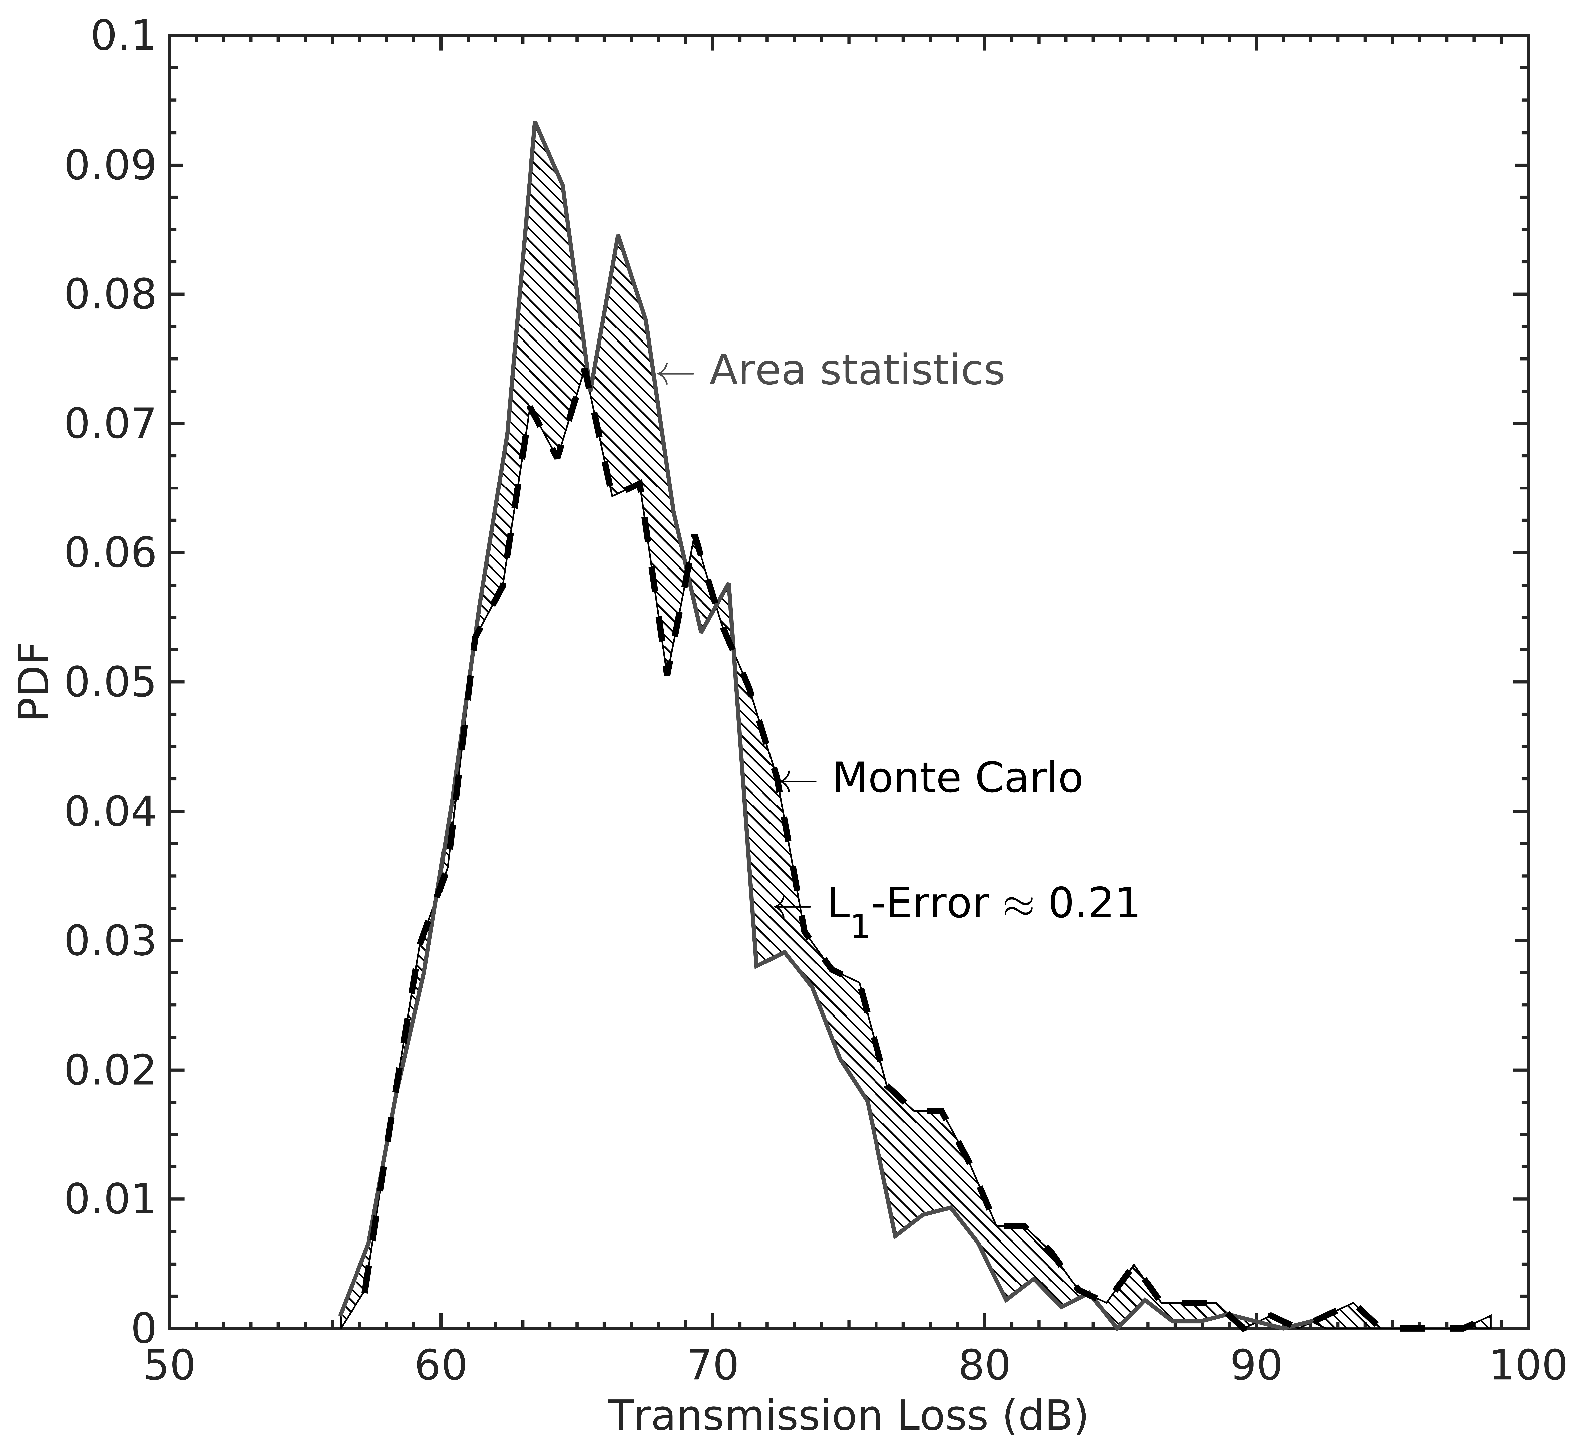
\includegraphics[width=0.47\textwidth]{./figs/asuq_figs/4a}
  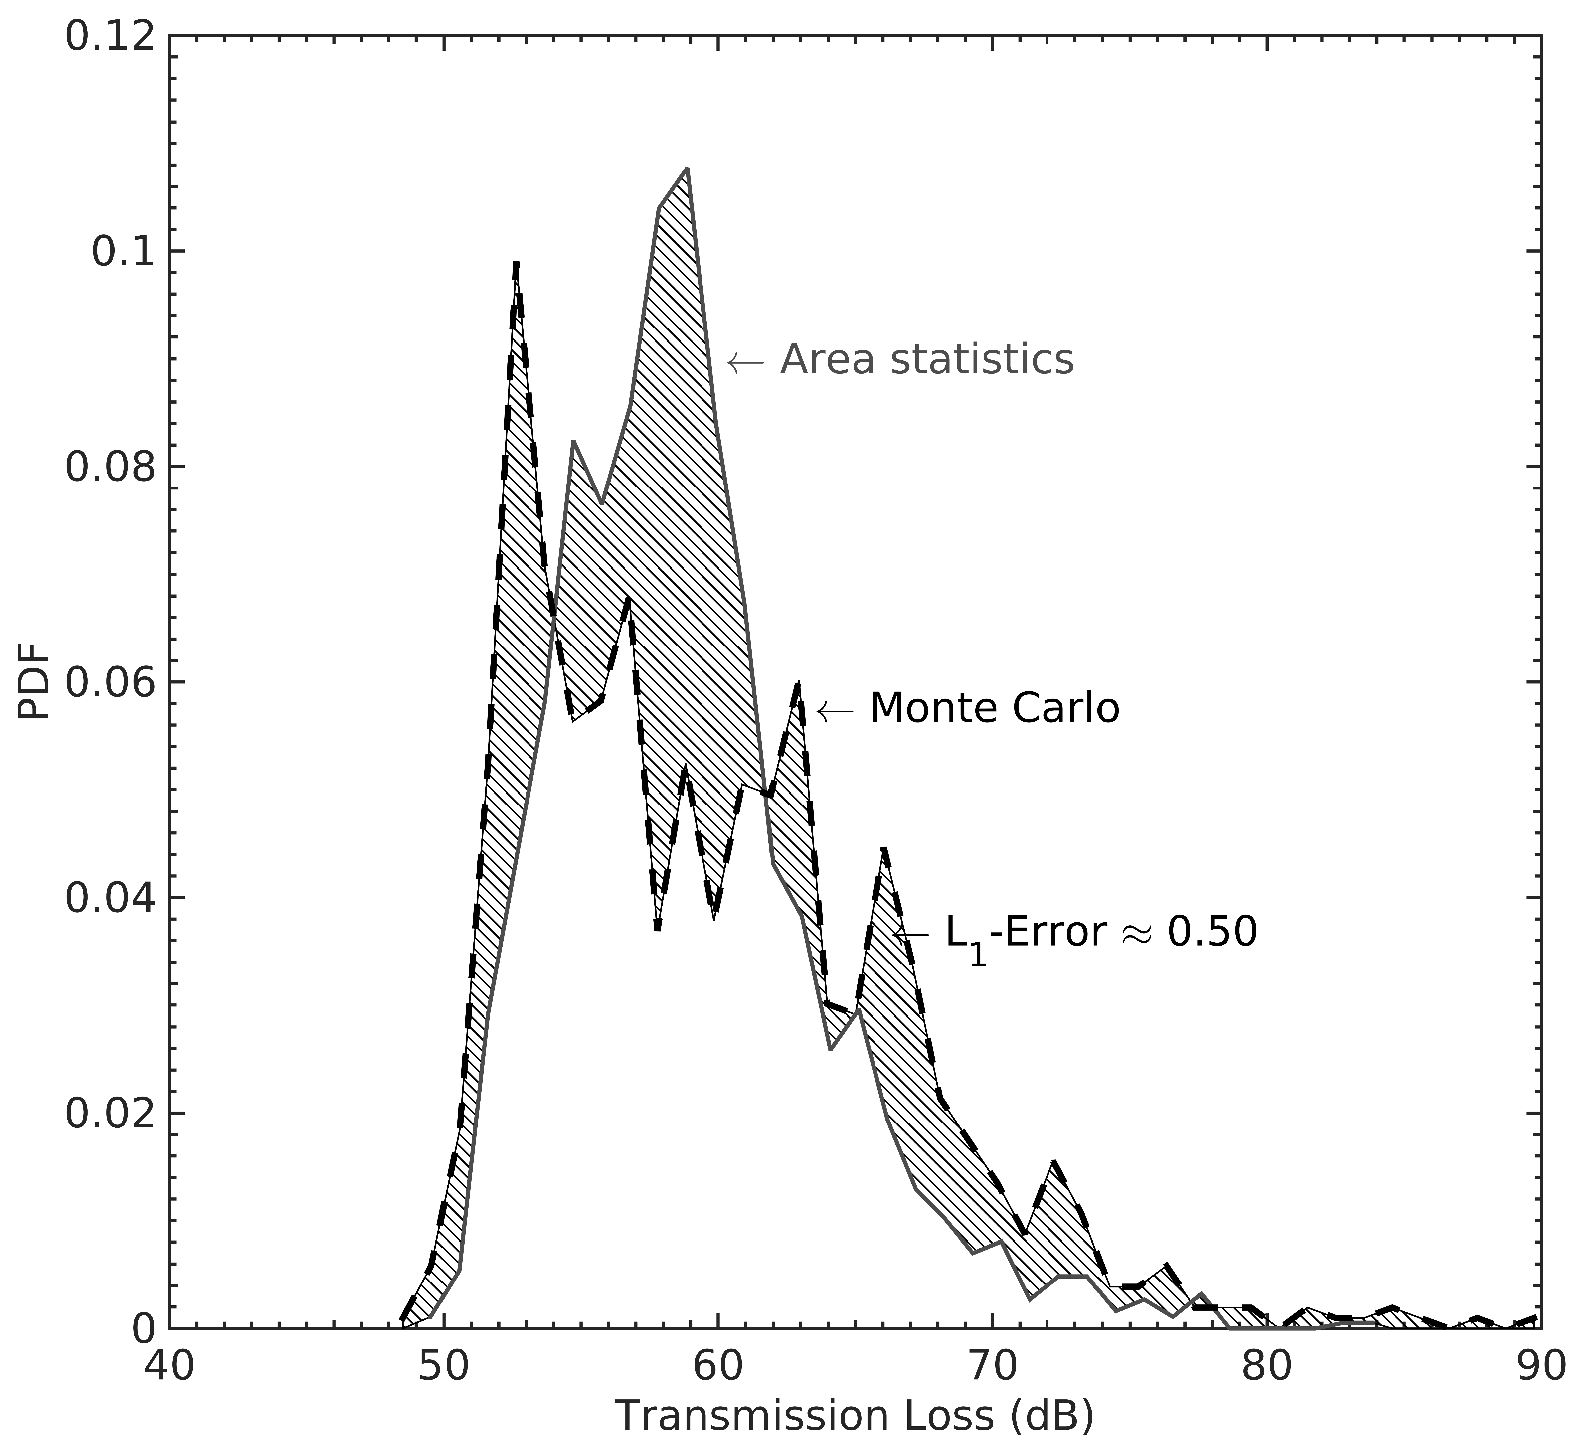
\includegraphics[width=0.47\textwidth]{./figs/asuq_figs/4b}
  \caption[Example acceptable and unacceptable Area
  statistics generated \acp{PDF} of \ac{TL} compared with their \ac{MC}
  counterparts.]{Comparison of area-statistics (solid curve) and
    \ac{MC} (dashed curve) generated \acp{PDF} of \ac{TL} in
    environment 2 at $r=5720$ m and $z=288$ m (a), and $r=1140$ m and
    $z=384$ m. In both panels, the $L_1$-error is the jagged marked
    area. (Left) $L_1=0.21$. With the \ac{MC} \ac{PDF} assumed to be
    correct, the mean and standard deviation errors of the area
    statistics \ac{PDF} is 1.23 dB and 1.02 dB, respectively. (Right)
    $L_1=0.503$. The mean and standard deviation errors are 0.86 dB
    and 1.92 dB, respectively. The area- statistics-estimated \ac{PDF}
    of \ac{TL} on the left is considered engineering-level accurate
    while that on the right is not.}
  \label{fig:asuq_astats_L1}
\end{figure}

\begin{figure}[htb]
  \centering
  \includegraphics[width=0.9\textwidth]{./figs/asuq_figs/5}
  \caption[\ac{TL} fields of each environment, with test locations
  shown, indicating where area statistics was and was not
  engineering-level accurate.]{\ac{TL} fields for the four
    environments shown in Figure \ref{fig:asuq_astats_bathy} with a
    $f_s=200$ Hz source and markers indicating locations where area
    statistics and \ac{MC} generated \acp{PDF} of \ac{TL} were
    compared. White circles indicate locations where area-statistics
    results compare favorably with those from \ac{MC} calculations
    ($L_1 \leq 0.50$). Black triangles indicate locations where such
    comparisons are unfavorable ($L_1 \geq 0.50$).}
  \label{fig:asuq_astats_field_results}
\end{figure}



\clearpage
\pagebreak

\section{Conclusions} \label{section:asuq_astats_conclusions} This
paper describes the area statistics technique for efficiently
estimating \ac{TL} uncertainty in underwater acoustics. The technique
is based on the idea that the \ac{TL} variation found near the point
interest in real space is similar to that found at the location of
interest when environmental parameters are varied. The technique is
simple and can be used to produce approximate \acp{PDF} of \ac{TL} in uncertain
ocean sound channels from a single (baseline) \ac{TL} field calculation
completed using the most probable value for each uncertain
parameter. To implement the technique, \ac{TL} values near a location of
interest in the baseline \ac{TL} field are collected and sorted into a
histogram that is normalized to obtain an approximate \ac{PDF} of \ac{TL} at the
location of interest. To determine the technique's accuracy, \acp{PDF} of
\ac{TL} created using area statistics were compared to \acp{PDF} generated using
1000-sample \ac{MC} calculations in four different ocean
environments at three acoustic frequencies ($f_s=100, 200, \text{and} 300$ Hz) for
three different source depths ($z_s=91, 137, \text{and} 183$m). The area-statistics
\acp{PDF} of \ac{TL} achieved engineering-level accuracy ($L_1\leq0.5$) in 93\% of
test cases in the three shallower environments with consistent bottom
reflection. In the environments where refraction was more important,
area statistics was less successful; engineering level accuracy was
only achieved in 56\% of test cases, initially.  However, this success
percentage was improved to 65\% by gently modifying the area
statistics algorithm, and this modification did not affect the results
in the shallower ocean environments.

The effort reported here supports the following four conclusions. (1)
The area statistics technique is a viable alternative, or worthy
complement, to \ac{MC} calculations or other more computationally
intensive techniques for estimating the uncertainty of \ac{TL} field
calculations in uncertain ocean environments with consistent
downward-refraction and bottom reflection. In each of the three
environments of this investigation meeting this bottom reflection
criterion, the technique produced engineering-level accuracy at 85\%
or more of the test locations. (2) The area statistics algorithm is
simple enough that it can be modified to improve the technique's
overall performance. One simple algorithm adjustment improved the
engineering accuracy success rate of area statistics in the deepest
environment considered in this study by approximately 10\% at all
three frequencies. (3) The area statistics technique is so inexpensive
computationally that it should be implemented even when a more
reliable but more computationally demanding approach is the primary
means for \ac{TL} uncertainty estimation. As part of this
investigation, the area statistics approach was found to be millions
of times faster than \ac{MC} calculations. Thus, the computational
penalty for implementing both, if the latter is preferred, is
vanishingly small. Moreover, the technique is computationally
inexpensive enough for use in real time applications. (4) The sample
rectangle size, \ac{TL} sample weighting, and other implementation
details of the area statistics algorithm described here are likely to
need adjustment if the ocean sound channel uncertainties of interest
differ from those considered. The area statistics technique is ad-hoc
and the implementation parameters in its current formulation were
tuned to achieve a high percentage of engineering-accurate predictions
for ocean sound channels with the uncertainties considered. However,
the uncertainties considered are generic and may serve as a useful
starting point for many uncertain ocean sound channels. Thus, the area
statistics formulation provided here may be broadly applicable.

%%% Local Variables:
%%% mode: latex
%%% TeX-master: "../../prelim"
%%% End:
